% import packages
\documentclass[8pt, table=xcolor,usenames,dvipsnames]{beamer}
\usepackage[utf8]{inputenc}
\usepackage{colortbl}
\usepackage{ragged2e}
\usepackage{booktabs}
\usepackage{threeparttable}
\usepackage{pifont}
\usepackage{graphicx}
\usepackage{hhline}
\usepackage{amsmath}
\usepackage{amssymb}
\usepackage{amsthm}
\usepackage{tikz}
\usepackage{bm}
\usepackage{etoolbox}
\usepackage[export]{adjustbox}
\usepackage[justification=centering]{caption}
\usepackage[backend=bibtex,style=authoryear,maxcitenames=2,natbib=true,maxbibnames=99]{biblatex}

% patch circles for framebreaks
% source: https://tex.stackexchange.com/a/132312
\makeatletter
\patchcmd{\slideentry}{\ifnum#2>0}{\ifnum2>0}{}{}
\patchcmd{\slideentry}{\c@subsectionslide}{\c@framenumber}{}{}
\patchcmd{\beamer@writeslidentry}{\c@subsectionslide}{\c@framenumber}{}{}
\makeatother

% set beamer parameters
\usetheme{Frankfurt}
\usecolortheme{default}
\setbeamerfont{footnote}{size=\Tiny}
\setbeamertemplate{page number in head/foot}{}
\setbeamertemplate{bibliography item}{}
\setbeamertemplate{caption}[numbered]
\setbeamercovered{transparent}
\setbeamerfont{institute}{size=\small}
\addtobeamertemplate{navigation symbols}{}{%
  \usebeamerfont{footline}%
  \usebeamercolor[fg]{footline}%
  \hspace{2em}%
  \raisebox{1.7pt}[0pt][0pt]{\insertframenumber/\inserttotalframenumber}
}
\setbeamertemplate{enumerate items}[square]
\setbeamertemplate{section in toc}[square]
\setbeamertemplate{theorems}[numbered]

% special command to uncover graphics
% source: https://tex.stackexchange.com/a/415335
\newcommand<>{\uncovergraphics}[2][{}]{
  % Taken from: <https://tex.stackexchange.com/a/354033/95423>
  \begin{tikzpicture}
    \node[anchor=south west,inner sep=0] (B) at (4,0)
    {\includegraphics[#1]{#2}}; \alt#3{}{%
      \fill [draw=none, fill=white, fill opacity=0.7] (B.north west) -- (B.north
      east) -- (B.south east) -- (B.south west) -- (B.north west) -- cycle; }
  \end{tikzpicture}
}

% set caption parameters
\DeclareCaptionFormat{myformat}{\fontsize{6}{6}\selectfont#1#2#3}
\captionsetup{format=myformat}
\captionsetup[figure]{labelfont={bf},name={Figure}}
\captionsetup[table]{labelfont={bf},name={Table}}

% set bibliography parameters
\renewcommand\refname{Bibliography}
\addbibresource{../bibtex.bib}
\setlength\bibitemsep{1.5\itemsep}
\let\oldcitep=\citep
\renewcommand\citep[1]{{\textcolor{blue}{\oldcitep{#1}}}}
\let\oldcitet=\citet
\renewcommand\citet[1]{{\textcolor{blue}{\oldcitet{#1}}}}

% miscellaneous settings
\settowidth{\leftmargini}{\usebeamertemplate{itemize item}}
\addtolength{\leftmargini}{\labelsep}
\renewcommand{\arraystretch}{1.3}
\graphicspath{{../visuals/}}
\newcolumntype{L}[1]{>{\RaggedRight\hspace{0pt}}p{#1}}

% set admin details
\title{Language detection using character n-gram profiles}
\subtitle{Inspiration from Cavnar and Trenkle (1994)}
\author{Atreya Shankar \\ Applying for: Scientific Researcher in NLP}
\date{July 6, 2021}

% start presentation
\begin{document}
\begin{frame}
  \maketitle
\end{frame}

\begin{frame}
  \frametitle{Overview}
  \tableofcontents
\end{frame}

\section{Introduction}

\begin{frame}
  \frametitle{Motivation}
  \begin{figure}
    \centering
    \begin{tikzpicture}
      \setlength{\fboxsep}{1pt}
      \node[anchor=south west,inner sep=0] at (0,0) {
        \fbox{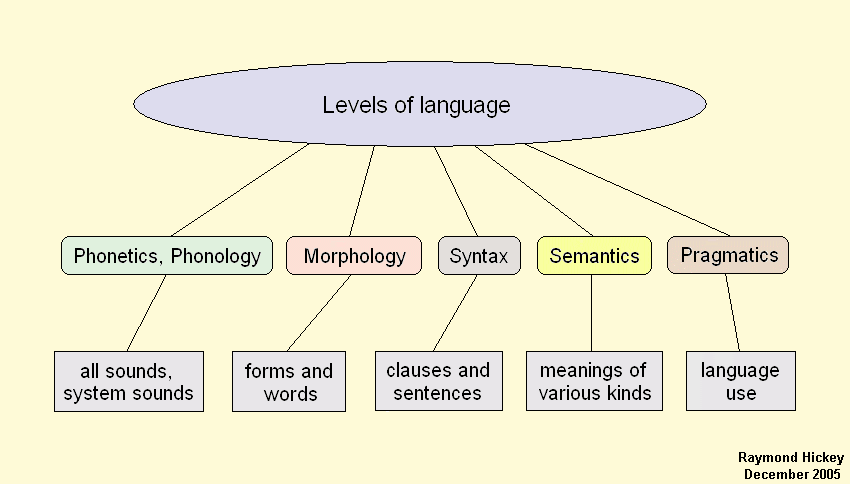
\includegraphics[width=9cm]{levels.png}}};
      \draw<2->[red, thick] (3,2.2) rectangle (4.6,2.75);
    \end{tikzpicture}
    \caption{Levels/structures of languages; figure taken from \citet{hickey2005levels}}
  \end{figure}
  \uncover<3>{\begin{itemize}
    \item Morphological profiling probably has lower data and compute requirements
    \item Makes sense given no external libraries are allowed
  \end{itemize}}
\end{frame}

\section{Methodology}

\begin{frame}
  \frametitle{Methodology}
\end{frame}

\section{Results}

\begin{frame}
  \frametitle{Results}
\end{frame}

\section{Discussion}

\begin{frame}
  \frametitle{Discussion}
\end{frame}

\section{Conclusions}

\begin{frame}
  \frametitle{Conclusions}
\end{frame}

\section*{Bibliography}

\begin{frame}[allowframebreaks]
  \frametitle{Bibliography}
  \nocite{*}
  \printbibliography[title = {Bibliography}, heading=none]
\end{frame}

\end{document}